% ------------------------------------------------------------------------------
% TYPO3 CMS 6.2 LTS - What's New - Chapter "TypoScript" (French version)
%
% @author	Paul Blondiaux <pblondiaux@sodifrance.fr>
% @author	Philippe Herault <philippe.herault@plan-net.fr>
% @license	Creative Commons BY-NC-SA 3.0
% @link		http://typo3.org/download/release-notes/whats-new/
% @language	French
% ------------------------------------------------------------------------------
% Chapter: TypoScript
% ------------------------------------------------------------------------------

\section{TSconfig \& TypoScript}
\begin{frame}[fragile]
	\frametitle{TSconfig \& TypoScript}

	\begin{center}\huge{Chapitre 4 :}\end{center}
	\begin{center}\huge{\color{typo3darkgrey}\textbf{TSconfig \& TypoScript}}\end{center}

\end{frame}

% ------------------------------------------------------------------------------
% Include TypoScript
% ------------------------------------------------------------------------------
% http://forge.typo3.org/issues/34621

\begin{frame}[fragile]
	\frametitle{TSconfig \& TypoScript}
	\framesubtitle{Inclusions TypoScript (1)}

	\begin{itemize}
		\item Inclusion de tous les fichiers TypoScript d'un répertoire (récursif)

			\lstinline!<INCLUDE_TYPOSCRIPT: source="DIR:directory">!
			\lstinline!<INCLUDE_TYPOSCRIPT: source="DIR:EXT:myextension/res/setup">!

		\item Ordre d'inclusion des fichiers :\newline
			par ordre alphabétique, d'abord les fichiers, puis les répertoires
		\item Limitation des fichiers à inclure en ajoutant \texttt{extensions="..."}

			\lstinline!<INCLUDE_TYPOSCRIPT: source="DIR:directory" extensions="ts">!

		\item Par défaut, seuls les fichiers avec les extensions : ts, t3, t3s, t3c, txt peuvent être inclus
		\item Cette liste est configurable (Install Tool) :\newline
			\texttt{\$TYPO3\_CONF\_VARS['SYS']['tsfile\_ext']}
	\end{itemize}

\end{frame}

% ------------------------------------------------------------------------------
% Include TypoScript
% ------------------------------------------------------------------------------
% http://forge.typo3.org/issues/52018

\begin{frame}[fragile]
	\frametitle{TSconfig \& TypoScript}
	\framesubtitle{Inclusions TypoScript (2)}

	\begin{itemize}
		\item Les chemins relatifs peuvent être passés à \texttt{INCLUDE\_TYPOSCRIPT}\newline
			si l'inclusion est appellée récursivement depuis un fichier
		\item La première inclusion \textbf{doit être} absolue
		\item \texttt{./} répertoire de la dernière inclusion
		\item \texttt{../} répertoire parent de la dernière inclusion
		\item Exemples:

			\lstinline!<INCLUDE_TYPOSCRIPT: source="FILE:directory/typoscript/setup.ts">!
			\lstinline!<INCLUDE_TYPOSCRIPT: source="FILE:./filename.ts">!
			\lstinline!<INCLUDE_TYPOSCRIPT: source="FILE:../filename.ts">!
			\lstinline!<INCLUDE_TYPOSCRIPT: source="FILE:../directory/filename.ts">!

	\end{itemize}

\end{frame}

% ------------------------------------------------------------------------------
% stdWrap for strPad
% ------------------------------------------------------------------------------
% http://forge.typo3.org/issues/43604

\begin{frame}[fragile]
	\frametitle{TSconfig \& TypoScript}
	\framesubtitle{strPad}

	\begin{itemize}
		\item L'option \texttt{stdWrap} a été ajoutée aux propriétés de \texttt{strPad}

			\begin{lstlisting}
				page = PAGE
				page.10 = TEXT
				page.10 {
				  value = Hello World!
				  strPad {
				    length = 5
				    length {
				      current = 1
				      setCurrent.data = TSFE:page|uid
				      setCurrent.wrap = | + 80
				      prioriCalc = 1
				    }
				    padWith = .
				  }
				}
			\end{lstlisting}

	\end{itemize}

\end{frame}

% ------------------------------------------------------------------------------
% stdWrap for _DEFAULT_PI_VARS
% ------------------------------------------------------------------------------
% http://forge.typo3.org/issues/22045
% http://forge.typo3.org/issues/49314

\begin{frame}[fragile]
	\frametitle{TSconfig \& TypoScript}
	\framesubtitle{\_DEFAULT\_PI\_VARS}

	\begin{itemize}
		\item \texttt{stdWrap} a été ajouté à \texttt{\_DEFAULT\_PI\_VARS}
		\item \texttt{\_DEFAULT\_PI\_VARS} permettent de paramétrer les valeurs par défaut pour piVars (Variables GET/POST d'une extension)

		\item TYPO3 < 6.2
			\begin{lstlisting}
				plugin.tt_news._DEFAULT_PI_VARS {
				  year = 2013
				}
			\end{lstlisting}

		\item TYPO3 >= 6.2
			\begin{lstlisting}
				plugin.tt_news._DEFAULT_PI_VARS {
				  year.stdWrap.data = date:Y
				}
			\end{lstlisting}

	\end{itemize}

\end{frame}

% ------------------------------------------------------------------------------
% Debug Register and Page
% ------------------------------------------------------------------------------
% http://forge.typo3.org/issues/49478

\begin{frame}[fragile]
	\frametitle{TSconfig \& TypoScript}
	\framesubtitle{Sortie de débogage}

	\begin{columns}[T]

		\begin{column}{.6\textwidth}
			\begin{itemize}
				\item Débogage pour les pages et variables déclarées :\newline
					\texttt{\$GLOBALS['TSFE']->register}\newline
					\texttt{\$GLOBALS['TSFE']->page}

				\item Exemples :

					\begin{lstlisting}
						10 = LOAD_REGISTER
						10.variable = value
					\end{lstlisting}

					\begin{lstlisting}
						20 = TEXT
						20.data = debug:register
					\end{lstlisting}

					\begin{lstlisting}
						30 = TEXT
						30.data = debug:page
					\end{lstlisting}

			\end{itemize}
		\end{column}

		\begin{column}{.4\textwidth}
			\begin{figure}\vspace*{-0.4cm}
				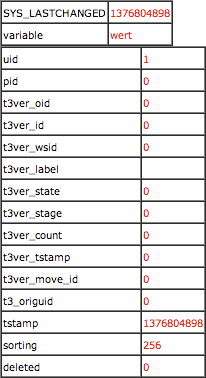
\includegraphics[width=0.6\linewidth]{Images/TypoScript/DebugRegisterAndPage.png}
			\end{figure}
		\end{column}

	\end{columns}

\end{frame}

% ------------------------------------------------------------------------------
% File Links: "register:titleText" and "register:altText"
% ------------------------------------------------------------------------------
% http://forge.typo3.org/issues/44182

\begin{frame}[fragile]
	\frametitle{TSconfig \& TypoScript}
	\framesubtitle{Liens Fichiers}

	\begin{itemize}
		\item Le contenu « liste de fichiers » offre une description, un titre et une alternative textuelle pour chaque fichier.
			Tous trois sont accessibles via les « registers » :

			\begin{itemize}
				\item \texttt{register:description}
				\item \texttt{register:titleText}
				\item \texttt{register:altText}
			\end{itemize}

		\item Exemple :

			\begin{lstlisting}
				# filelinks
				tt_content.uploads.20 {
				  # link description instead of filename
				  labelStdWrap.data = register:description
				  # output alternative text
				  itemRendering.20.data = register:titleText
				}
			\end{lstlisting}

	\end{itemize}

\end{frame}

% ------------------------------------------------------------------------------
% stdWrap replacement: add optionSplit-support
% ------------------------------------------------------------------------------
% http://forge.typo3.org/issues/42287

\begin{frame}[fragile]
	\frametitle{TSconfig \& TypoScript}
	\framesubtitle{Fonction stdWrap : replacement (1)}

	\begin{itemize}
		\item L'option \texttt{replace} de la fonction \texttt{stdWrap} \texttt{replacement}\newline
			supporte maintenant les \texttt{optionSplit}

		\item Exemple 1 :

			\begin{lstlisting}
				10 = TEXT
				10.value = TYPO3_inspires_people_to_share
				10.replacement.10 {
				  search = _
				  replace = 1 || 2 || 3
				  useOptionSplitReplace = 1
				}
			\end{lstlisting}

			Sortie :\newline
				\texttt{TYPO31inspires2people3to3share}

	\end{itemize}

\end{frame}

% ------------------------------------------------------------------------------
% stdWrap replacement: add optionSplit-support
% ------------------------------------------------------------------------------
% http://forge.typo3.org/issues/42287

\begin{frame}[fragile]
	\frametitle{TSconfig \& TypoScript}
	\framesubtitle{Fonction stdWrap : replacement (2)}

	\begin{itemize}

		\item Exemple 2 :

			\begin{lstlisting}
				10 = TEXT
				10.value = TYPO3 inspires people to share
				10.replacement.10 {
				  search = #(TYPO3|people|share)#i
				  replace = ${1} CMS || all ${1} || collaborate and ${1}
				  useOptionSplitReplace = 1
				  useRegExp = 1
				}
			\end{lstlisting}

			Sortie :\newline
				\texttt{TYPO3 CMS inspires all people to collaborate and share}

	\end{itemize}

\end{frame}

% ------------------------------------------------------------------------------
% Register values in FilesContentObject
% ------------------------------------------------------------------------------
% http://forge.typo3.org/issues/49480

\begin{frame}[fragile]
	\frametitle{TSconfig \& TypoScript}
	\framesubtitle{cObject FILE}

	\begin{itemize}
		\item Deux « registers » ont été ajoutés au cObject « FILES » :\newline
			\texttt{FILE\_NUM\_CURRENT} et \texttt{FILES\_COUNT}

		\item Exemple :

			\lstset{
				basicstyle=\tiny\ttfamily
			}

			\begin{lstlisting}
				10 = FILES
				10 {
				  references {
				    table = tt_news
				    uid.field = uid
				    fieldName = media
				  }
				  renderObj = COA
				  renderObj {
				    10 = TEXT
				    10.value = Renders first file twice
				    10.if.isFalse.data = register:FILE_NUM_CURRENT
				    20 = TEXT
				    20.value = file {register:FILE_NUM_CURRENT} of {register:FILES_COUNT}
				    20.insertData = 1
				  }
				}
			\end{lstlisting}

	\end{itemize}

\end{frame}

% ------------------------------------------------------------------------------
% Category Menu In TypoScript
% ------------------------------------------------------------------------------
% http://forge.typo3.org/issues/51161

\begin{frame}[fragile]
	\frametitle{TSconfig \& TypoScript}
	\framesubtitle{Menu de catégories}

	\begin{itemize}
		\item Générer un menu de catégories en TypoScript

		\item Exemple :

			\lstset{
				basicstyle=\tiny\ttfamily
			}

			\begin{lstlisting}
				page.20 = HMENU
				page.20 {
				  special = categories
				  special {
				    # comma-separated list of categories
				    value = 1
				    # sort by title (stdWrap)
				    sorting = title
				    # sorting "asc" or "desc" (stdWrap)
				    order = desc
				    1 = TMENU
				    1.NO {
				      allWrap = <li> | </li>
				    }
				  }
				}
			\end{lstlisting}

	\end{itemize}

\end{frame}

% ------------------------------------------------------------------------------
% cObject RECORDS with category support
% (slide added in March 2014)
% ------------------------------------------------------------------------------

\begin{frame}[fragile]
	\frametitle{TSconfig \& TypoScript}
	\framesubtitle{Accès aux catégories}

	\begin{itemize}
		\item La propriété \texttt{categories} permet d'accéder aux catégories\newline
			du cObject RECORDS

		\item Exemple :

			\lstset{
				basicstyle=\tiny\ttfamily
			}

			\begin{lstlisting}
				# menu of categorized content elements
				categorized_content = RECORDS
				categorized_content {
				  categories.field = selected_categories
				  categories.relation.field = category_field
				  tables = tt_content
				  conf.tt_content = TEXT
				  conf.tt_content {
				    field = header
				    typolink.parameter = {field:pid}#{field:uid}
				    typolink.parameter.insertData = 1
				    wrap = <li>|</li>
				  }
				  wrap = <ul>|</ul>
				}
			\end{lstlisting}

	\end{itemize}

\end{frame}

% ------------------------------------------------------------------------------
% Category Menu In TypoScript
% ------------------------------------------------------------------------------
% http://forge.typo3.org/issues/51782

\begin{frame}[fragile]
	\frametitle{TSconfig \& TypoScript}
	\framesubtitle{Fichiers CSS et JavaScript}

	\begin{itemize}
		\item \texttt{splitChar} peut maintenant être défini pour les propriétés \texttt{allWrap}
		\item Le « wrap » fonctionne maintenant comme la méthode standard \texttt{stdWrap.wrap}
		\item Le caractère \texttt{splitChar} par défaut est le symbole « pipe » : \texttt{|}
		\item Ce changement affecte :

			\begin{itemize}
				\item \texttt{includeCSS}
				\item \texttt{includeJSlibs}
				\item \texttt{includeJSFooterlibs}
				\item \texttt{includeJS}
				\item \texttt{includeJSFooter}
			\end{itemize}

	\end{itemize}

\end{frame}

% ------------------------------------------------------------------------------
% Conditions: userFunc Accepts Multiple Arguments
% ------------------------------------------------------------------------------
% http://forge.typo3.org/issues/47159

\begin{frame}[fragile]
	\frametitle{TSconfig \& TypoScript}
	\framesubtitle{Conditions (1)}

	\begin{itemize}
		\item La condition \texttt{userFunc} accepte maintenant des arguments multiples

		\item TYPO3 < 6.2
			\begin{lstlisting}
				[userFunc = user_function(argument1)]
			\end{lstlisting}

		\item TYPO3 >= 6.2
			\begin{lstlisting}
				[userFunc = user_function(argument1, argument2, ...)]
			\end{lstlisting}

		\item Exemple :
			% \texttt{[userFunc = user\_match(checkSubnet, 192.168)]}

			\lstinline![userFunc = user_match(checkSubnet, 192.168)]!

			\begin{lstlisting}
				function user_match($command, $subnet) {
				  switch($command) {
				    case 'checkSubnet':
				      if (strstr(getenv('REMOTE_ADDR'), $subnet)) { ... }
				  }
				}
			\end{lstlisting}

	\end{itemize}

\end{frame}

% ------------------------------------------------------------------------------
% Conditions: Application Context
% ------------------------------------------------------------------------------
% http://forge.typo3.org/issues/39441
% http://forge.typo3.org/issues/50132

\begin{frame}[fragile]
	\frametitle{TSconfig \& TypoScript}
	\framesubtitle{Conditions (2)}

	\begin{itemize}
		\item Le contexte de l'application peut être déterminé dans les conditions
		\item Les « wildcards » « \texttt{+} » et « \texttt{*} », et les expressions régulières sont supportés
		\item Exemple :

			\lstset{
				basicstyle=\tiny\ttfamily
			}

			\begin{lstlisting}
				[applicationContext = Development/Debugging, Development/Profiling]
				  # TYPO3 site in development stage
				[global]

				[applicationContext = Production*]
				  # TYPO3 site in production stage
				  # for example "Production/Live" or "Production/Staging"
				[global]

				[applicationContext = /^TestServer\d+$/]
				  # TYPO3 site on TestServer1 or TestServer2 or TestServer3, etc.
				[global]
			\end{lstlisting}

	\end{itemize}

\end{frame}

% ------------------------------------------------------------------------------
% Conditions: IP Supports Keyword devIP
% ------------------------------------------------------------------------------
% http://forge.typo3.org/issues/50092

\begin{frame}[fragile]
	\frametitle{TSconfig \& TypoScript}
	\framesubtitle{Conditions (3)}

	\begin{itemize}

		\item Lors de l'utilisation d'une condition sur l'IP, le mot-clé \texttt{devIP} peut\newline
			être utilisé pour vérifier si l'IP du client correspond au\newline
			paramétrage de \texttt{devIpMask} dans l'Install Tool
		\item Exemple :

%			\lstset{
%				basicstyle=\tiny\ttfamily
%			}

			\begin{lstlisting}
				[IP = devIP]
				  page.10 = TEXT
				  page.10.value = Hello Developer!
				[global]
			\end{lstlisting}

	\end{itemize}

\end{frame}

% ------------------------------------------------------------------------------
% Records Without Default Translation
% ------------------------------------------------------------------------------
% http://forge.typo3.org/issues/24005

\begin{frame}[fragile]
	\frametitle{TSconfig \& TypoScript}
	\framesubtitle{Enregistrements sans traduction par défaut}

	\begin{itemize}

		\item La nouvelle option \texttt{includeRecordsWithoutDefaultTranslation}
			récupére les enregistrements dépourvus de parents localisés\newline
			(mais avec le champ \texttt{languageField} correspondant au langage courant)

		\item Exemple :

			\begin{lstlisting}
				pageContent = CONTENT
				pageContent {
				  table = tt_content
				  select.includeRecordsWithoutDefaultTranslation = 1
				  ...
				}
			\end{lstlisting}

	\end{itemize}

\end{frame}

% ------------------------------------------------------------------------------
% cObject FILES: begin/maxItems options
% ------------------------------------------------------------------------------
% http://forge.typo3.org/issues/52632

\begin{frame}[fragile]
	\frametitle{TSconfig \& TypoScript}
	\framesubtitle{cObject FILES}

	\begin{itemize}

		\item Le cObject FILES supporte maintenant les propriétés \texttt{begin} et \texttt{maxItems} 

		\item Exemple :

			\lstset{
				basicstyle=\tiny\ttfamily
			}

			\begin{lstlisting}
				page.10 = FILES
				page.10 {
				  references {
				    table = pages
				    uid.data = page:uid
				    fieldName = media
				  }

				  # retrieve up to 5 files, beginning at the first (0):
				  begin = 0
				  maxItems = 5

				  renderObj = TEXT
				  renderObj {
				    data = file:current:size
				    wrap = <p>File size:<strong>|</strong></p>
				  }
				}
			\end{lstlisting}

	\end{itemize}

\end{frame}

% ------------------------------------------------------------------------------
% Exclude doktypes From Pagetree
% ------------------------------------------------------------------------------
% http://forge.typo3.org/issues/49279
% http://forge.typo3.org/issues/49356

\begin{frame}[fragile]
	\frametitle{TSconfig \& TypoScript}
	\framesubtitle{Exclure des doktypes de l'arborescence}

	\begin{itemize}

		\item Des « doktypes » spécifiques peuvent être exclus de l'arborescence
		\item La configuration est à faire dans UserTSconfig (donc sur un utilisateur ou un groupe spécifique)
		\item Exemples :

			\begin{lstlisting}
				# exclude "folder" pages
				options.pageTree.excludeDoktypes = 254

				# exclude "folder" and "standard" pages
				options.pageTree.excludeDoktypes = 254,1
			\end{lstlisting}

	\end{itemize}

\end{frame}

% ------------------------------------------------------------------------------
% Hide Modules In Backend
% ------------------------------------------------------------------------------

\begin{frame}[fragile]
	\frametitle{TSconfig \& TypoScript}
	\framesubtitle{Cacher des modules en Backend}

	\begin{itemize}

		\item Les modules peuvent être cachés en Backend
		\item Ceci n'a pas d'impact sur l'accès au module\newline
			(utilisez les ACL pour les utilisateurs et groupes BE pour restreindre l'accès)
		\item Exemples :

			\lstinline!options.hideModules = file, help!
			\lstinline!options.hideModules.web := addToList(func,info)!
			\lstinline!options.hideModules.system = BelogLog!

	\end{itemize}

\end{frame}

% ------------------------------------------------------------------------------
% Alternative Domain For Preview
% ------------------------------------------------------------------------------
% http://forge.typo3.org/issues/30889

\begin{frame}[fragile]
	\frametitle{TSconfig \& TypoScript}
	\framesubtitle{Domaine de prévisualisation}

	\begin{itemize}

		\item Un domaine alternatif peut être paramétré en PageTS pour prévisualiser les pages ou les sites
		\item Utile pour les sites multi-domaines
		\item Exemple :

			\lstinline!TCEMAIN.viewDomain = example.com!

	\end{itemize}

\end{frame}

% ------------------------------------------------------------------------------
% Conditions in Backend Layouts
% ------------------------------------------------------------------------------
% http://forge.typo3.org/issues/47588

\begin{frame}[fragile]
	\frametitle{TSconfig \& TypoScript}
	\framesubtitle{Conditions dans les dispositions du Backend}

	\begin{itemize}

		\item En Backend, les dispositions supportent maintenant les conditions
		\item Exemple :

			\lstset{
				basicstyle=\tiny\ttfamily
			}

			\begin{lstlisting}
				backend_layout {
				  colCount = 2
				  rowCount = 1
				  rows {
				    1 {
				      columns {
				        1.name = Main
				        1.colPos = 0
				        2.name = Right
				        2.colPos = 1
				      }
				    }
				  }
				}

				[PIDupinRootline = 123]
				  # remove right column in branch of page ID 123
				  backend_layout.rows.1.columns.2 >
				[global]
			\end{lstlisting}

	\end{itemize}

\end{frame}


% ------------------------------------------------------------------------------
% Miscellaneous
% ------------------------------------------------------------------------------
% http://forge.typo3.org/issues/34597 (showForgotPassword)
% http://forge.typo3.org/issues/50138 (showForgotPassword)
%
% http://forge.typo3.org/issues/19732 (Content-Length)
%
% http://forge.typo3.org/issues/16386 (Indexed Search) - wow: submitted 7 years ago :-)

\begin{frame}[fragile]
	\frametitle{TSconfig \& TypoScript}
	\framesubtitle{Divers}

	\begin{itemize}

		\item Activer/Désactiver le lien « Mot de passe oublié » avec l'option \small\texttt{showForgotPassword}\normalsize\newline
			(utile si plusieurs formulaires d'identification sont inclus par EXT:felogin sur une même page)

		\item La réponse HTTP inclut maintenant l'en-tête \texttt{Content-length} par défaut

			\begin{itemize}
				\item Accélère le rendu si le « pipelining » est activé dans Apache
				\item Configurable avec \texttt{config.enableContentLengthHeader}
			\end{itemize}

		\item La liste de résultats de l'extension indexed\_search a des propriétés \texttt{stdWrap} maintenant\newline
			(option : \texttt{plugin.tx\_indexedsearch.resultlist\_stdWrap})

	\end{itemize}

\end{frame}

% ------------------------------------------------------------------------------
